\documentclass[a4paper,11pt]{article}
\usepackage[utf8]{inputenc}
\usepackage{graphicx}
\usepackage[a4paper]{geometry} %pour les marges
\geometry{hscale=0.77,vscale=0.85,centering}

\title{Configuration de routeur Cisco}
\author{Groupe 1:}
\date{4 octobre 2016}
\begin{document}
\maketitle

\section{Introduction}
En suivant une certaine topologie (figure \ref{fig:topo}),
nous devions d'abord configurer le routeur qui nous était attribué pour que nous puissions envoyer des pings aux PC des autres membres de notre groupe,
c'est à dire aux PC faisant partie de notre VLAN.
Ensuite, il fallait configurer notre routeur pour pouvoir envoyer des pings aux PC faisant partie d'autres VLAN.
\begin{figure}
 \centering
 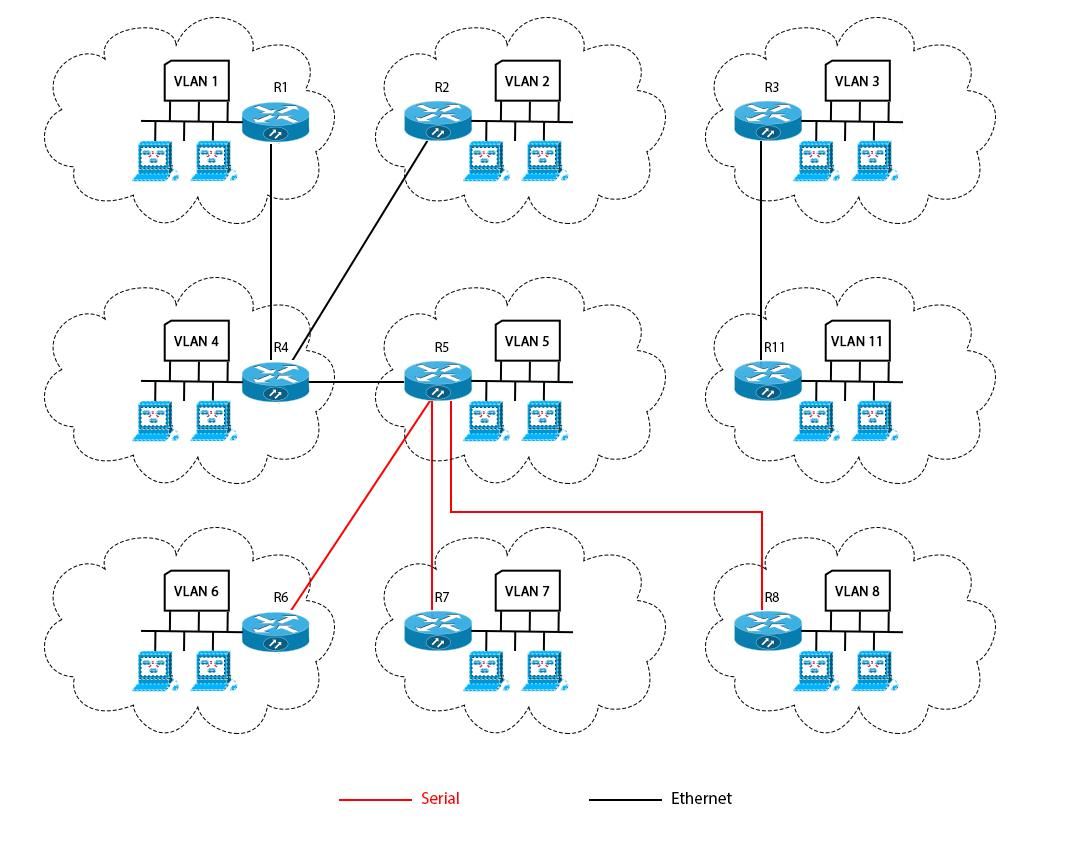
\includegraphics[height=7cm]{topo.jpg}
 \caption{Topologie à suivre pour ce travail pratique}
 \label{fig:topo}
\end{figure}


\end{document}